\documentclass[12pt,a4paper]{article}
\usepackage[T2A]{fontenc}
\usepackage[utf8]{inputenc}
\usepackage[russian,english]{babel}
\usepackage{amsmath, amssymb}
\usepackage{graphicx}
\usepackage{geometry}
\geometry{left=3cm,right=1.5cm,top=2cm,bottom=2cm}
\usepackage{float}
\usepackage{caption}
\usepackage{indentfirst}
\usepackage{titlesec}

% Section styling to match GOST/SPbPU 
\titleformat{\section}{\normalfont\large\bfseries}{\thesection.}{0.5em}{}
\titleformat{\subsection}{\normalfont\normalsize\bfseries}{\thesubsection.}{0.5em}{}

\sloppy

\begin{document}

% --- TITLE PAGE ---
\begin{titlepage}
    \centering
    Санкт-Петербургский Политехнический Университет Петра Великого\\
    Физико-Механический институт\\
    Высшая школа прикладной математики и вычислительной физики\\
    \vfill
    \textbf{Отчёт по лабораторной работе по дисциплине}\\
    \textbf{«Интервальный анализ»}\\
    \vfill
    \begin{flushright}
        Выполнил:\\
        студент гр. 5040102/40201\\
        \textbf{Стрижкин Д.А.}\\
        \vspace{1cm}
        Проверил:\\
        доцент\\
        \textbf{Баженов А.Н.}
    \end{flushright}
    \vfill
    Санкт-Петербург --- 2026
\end{titlepage}

\newpage
\section{Введение}
Радиус инверсии $R_{inv}$ является критическим параметром при анализе МГД-активности в плазме токамака Глобус-М2. Традиционные методы точечных оценок часто не учитывают погрешности измерений профилей температуры. В данной работе предлагается подход, основанный на интервальной регрессии и использовании индекса Жаккара.

\section{Теоретические основы интервальной статистики}
\subsection{Индекс Жаккара для профилей}
Для количественной оценки уровня доверия используется индекс Жаккара $J_I$:
\begin{equation}
    J_I(r) = \frac{wid(Te^{before}(r) \wedge Te^{after}(r))}{wid(Te^{before}(r) \vee Te^{after}(r))}
\end{equation}
где $\wedge$ и $\vee$ обозначают пересечение и объединение интервалов соответственно.

На основе анализа графика индекса Жаккара вводим две оценки:
\begin{enumerate}
    \item Внешняя оценка: $R_{ext} = \{r \mid J_I(r) > 0\}$.
    \item Внутренняя оценка: $R_{int} = \{r \mid J_I(r) > 0.5\}$.
\end{enumerate}

\section{Анализ данных токамака «Глобус-М2»}
На рис. \ref{fig:profiles} представлены типичные профили температуры до и после сброса пилообразного колебания с соответствующими коридорами неопределённости.

\begin{figure}[H]
    \centering
    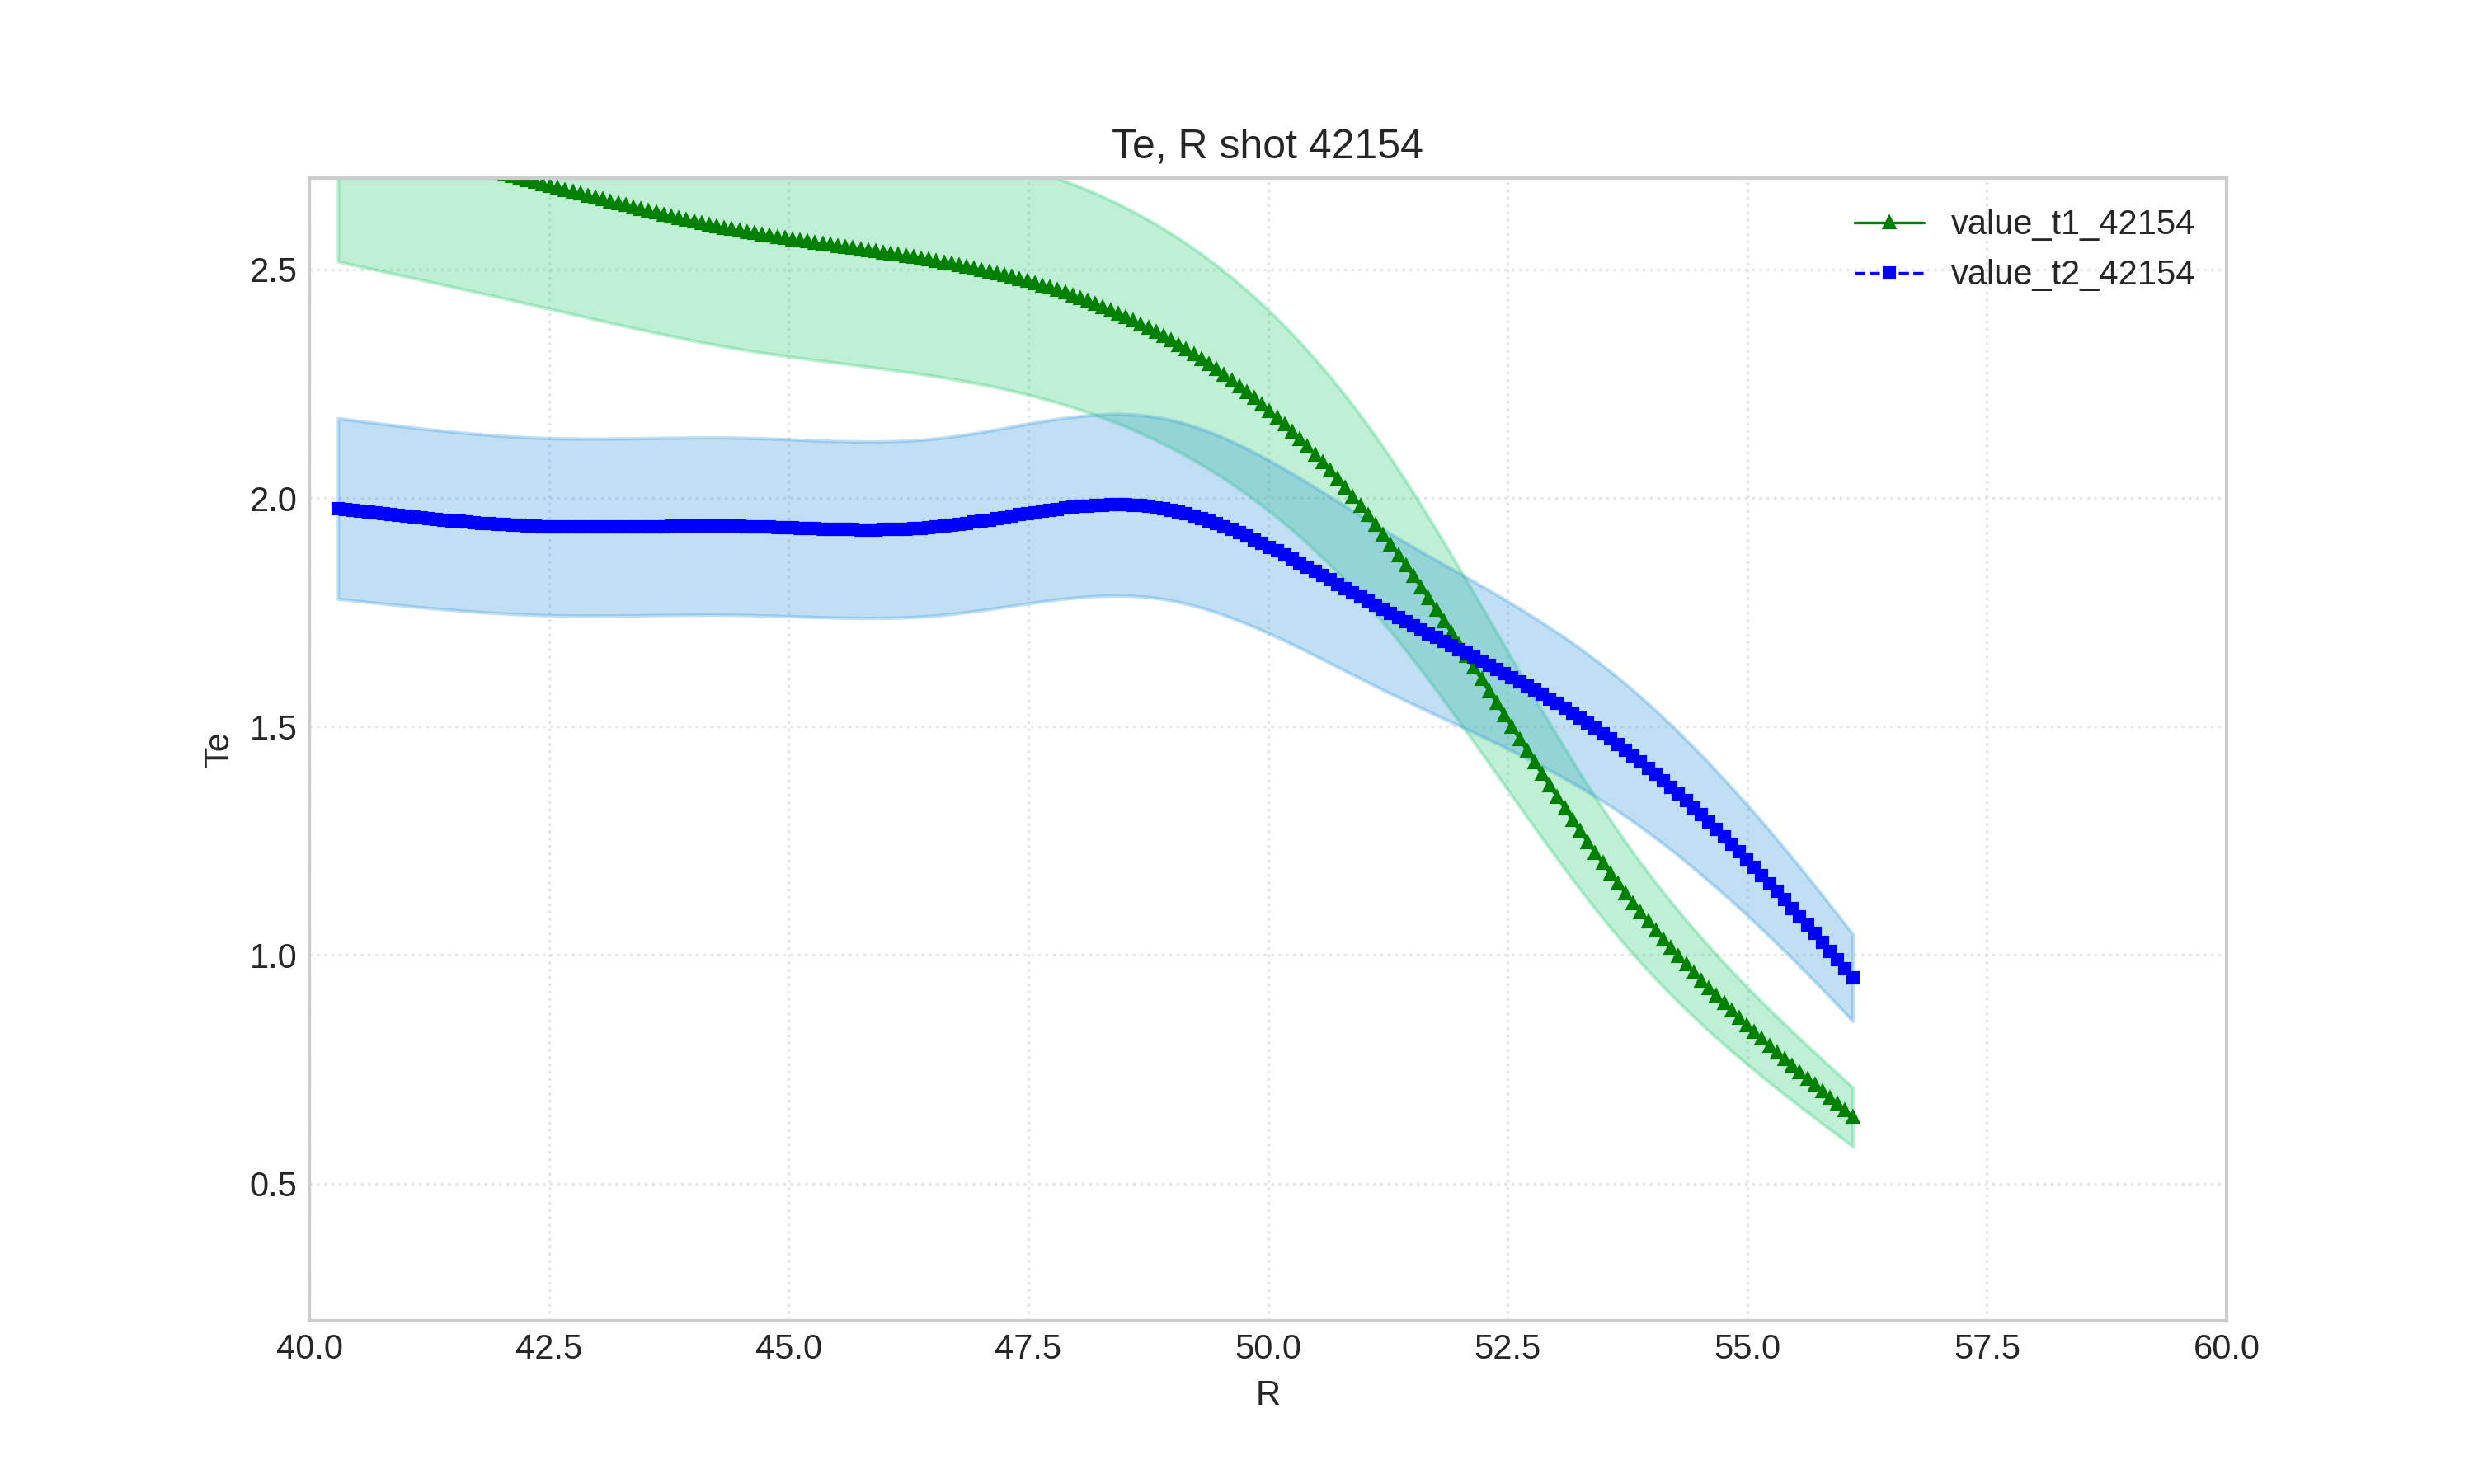
\includegraphics[width=0.8\textwidth]{images/fig_3_2_profiles.png}
    \caption{График температуры электронов от радиуса с коридорами.}
    \label{fig:profiles}
\end{figure}

Распределение индекса Жаккара для данного события показано на рис. \ref{fig:jaccard}.

\begin{figure}[H]
    \centering
    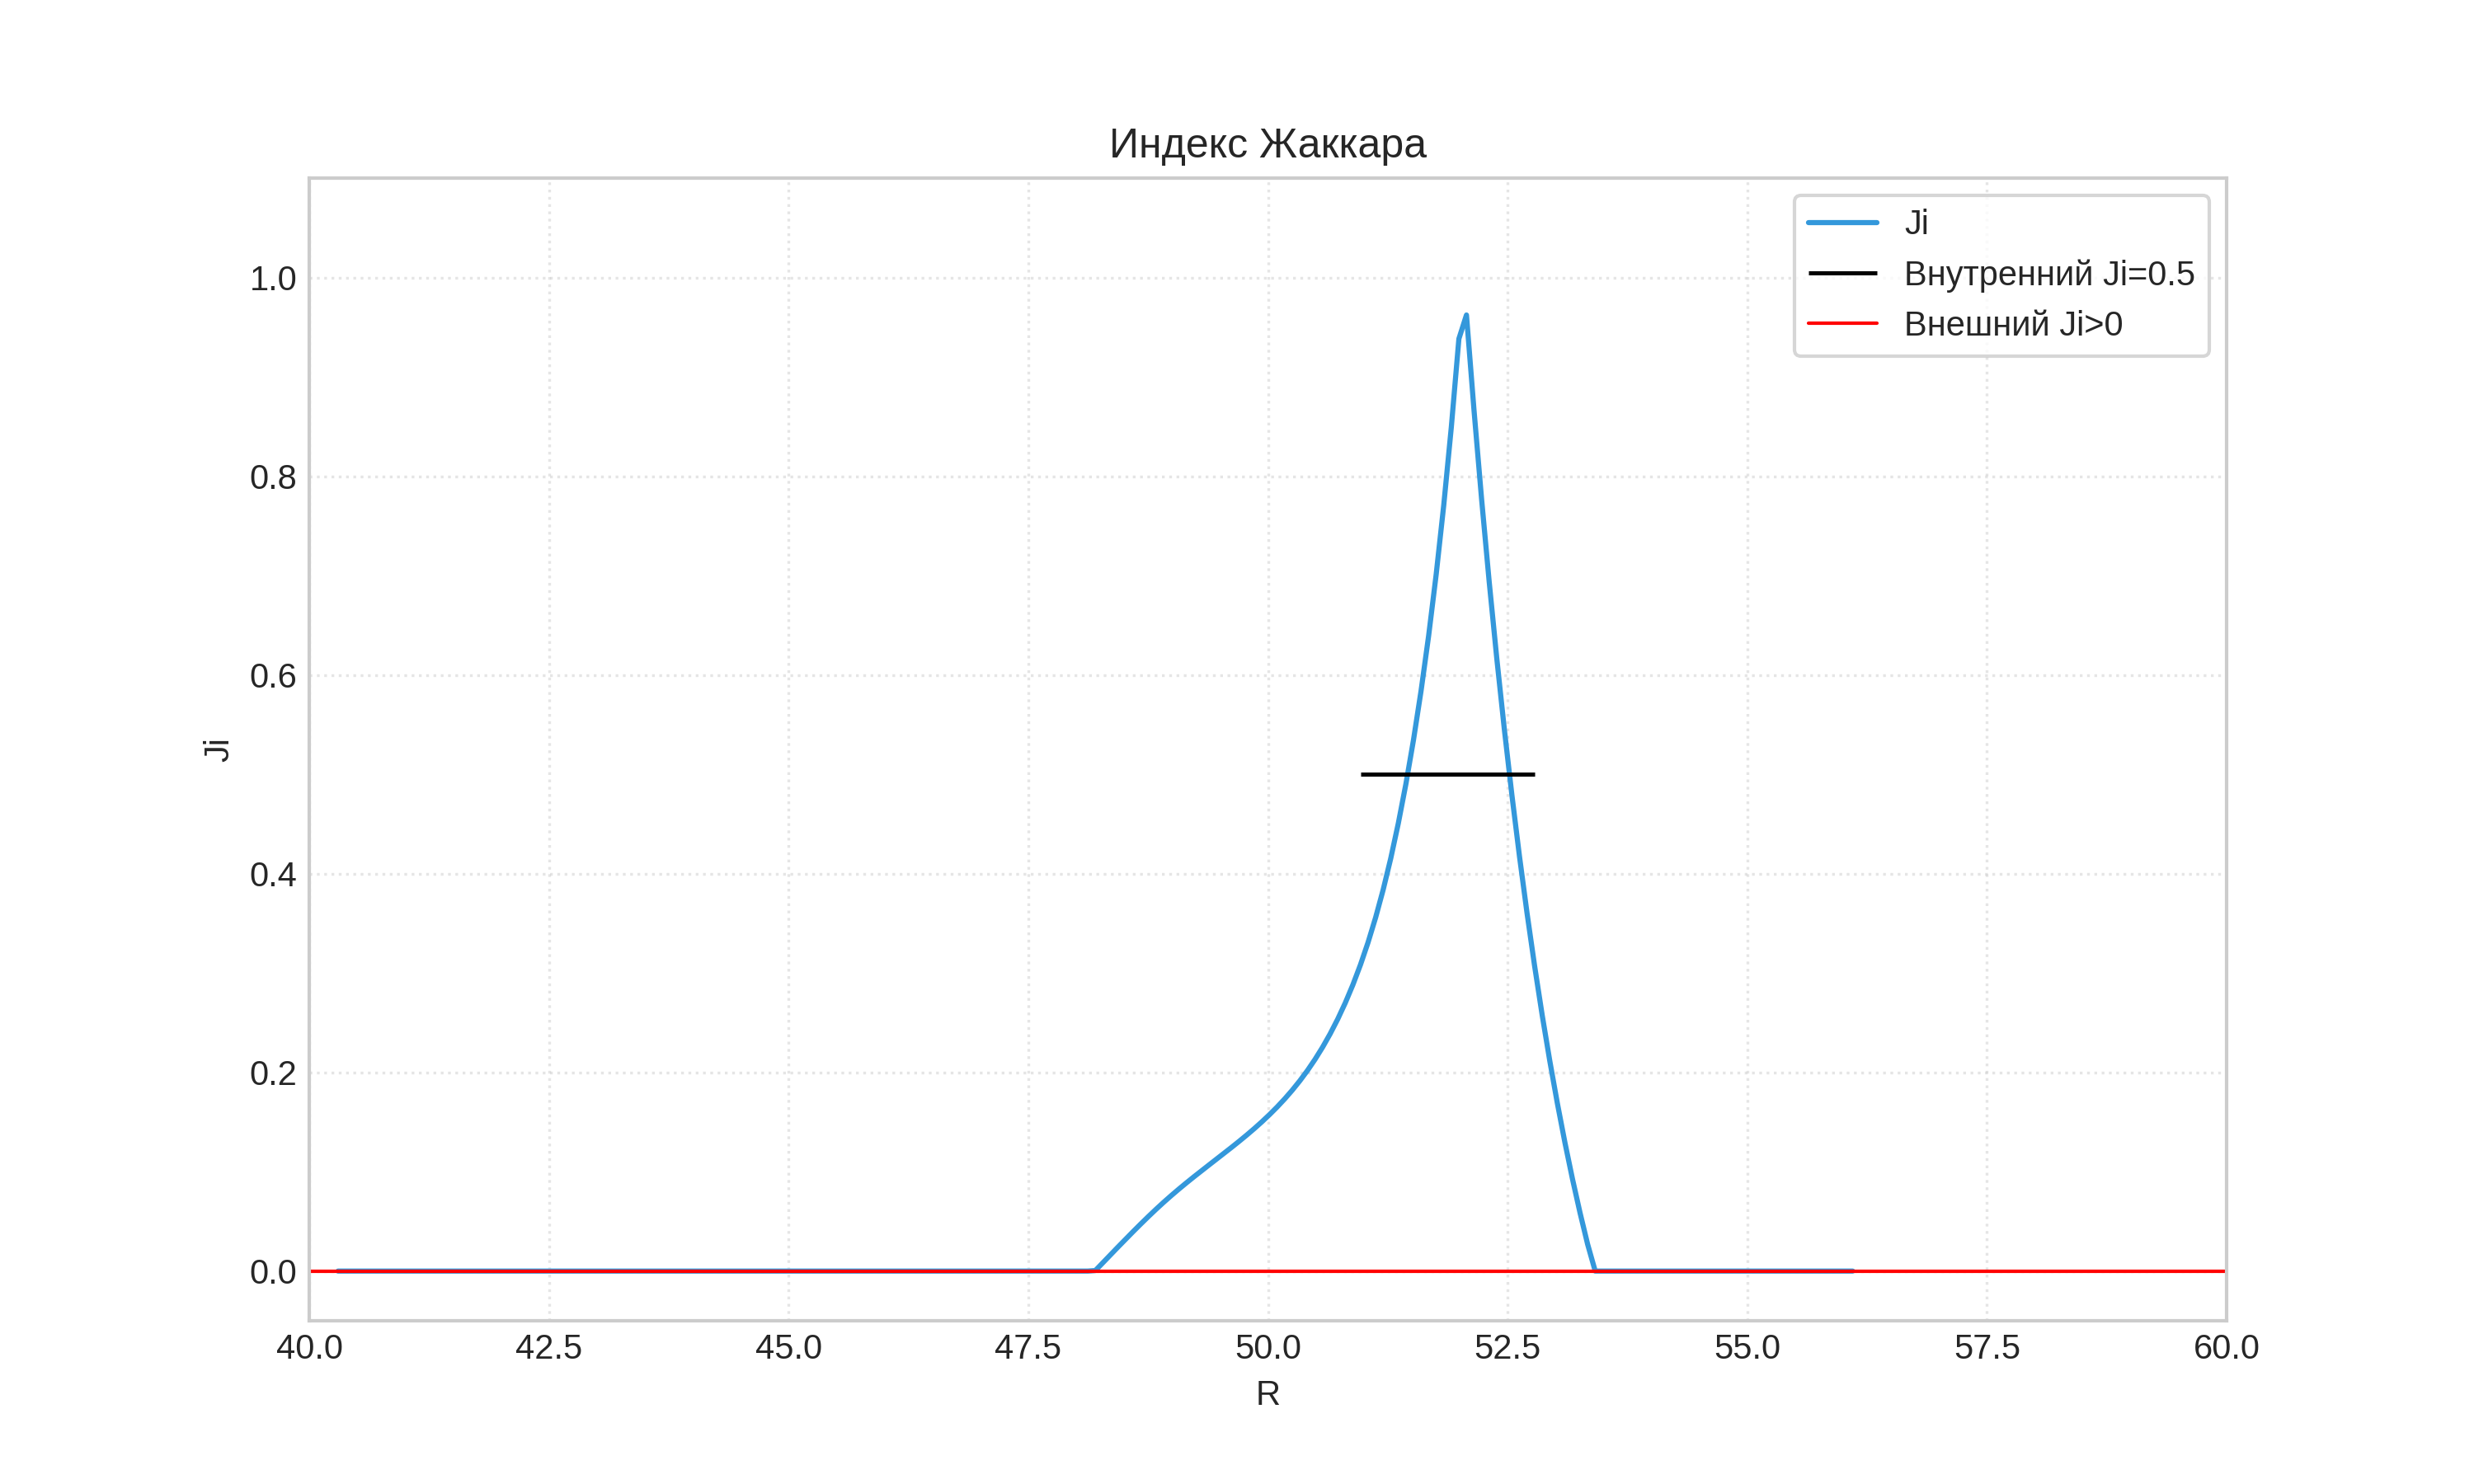
\includegraphics[width=0.8\textwidth]{images/fig_3_3_jaccard.png}
    \caption{Индекс Жаккара для пересекающихся коридоров.}
    \label{fig:jaccard}
\end{figure}

\section{Результаты и их интерпретация}
\subsection{Анализ полученных интервальных оценок}
Для каждого экспериментального значения параметра $B_T/I_P$ определен соответствующий интервал $R_{inv} \in [R_{min}, R_{max}]$.
На рис. \ref{fig:internal} и \ref{fig:external} представлены внутренние и внешние интервальные оценки соответственно.

\begin{figure}[H]
    \centering
    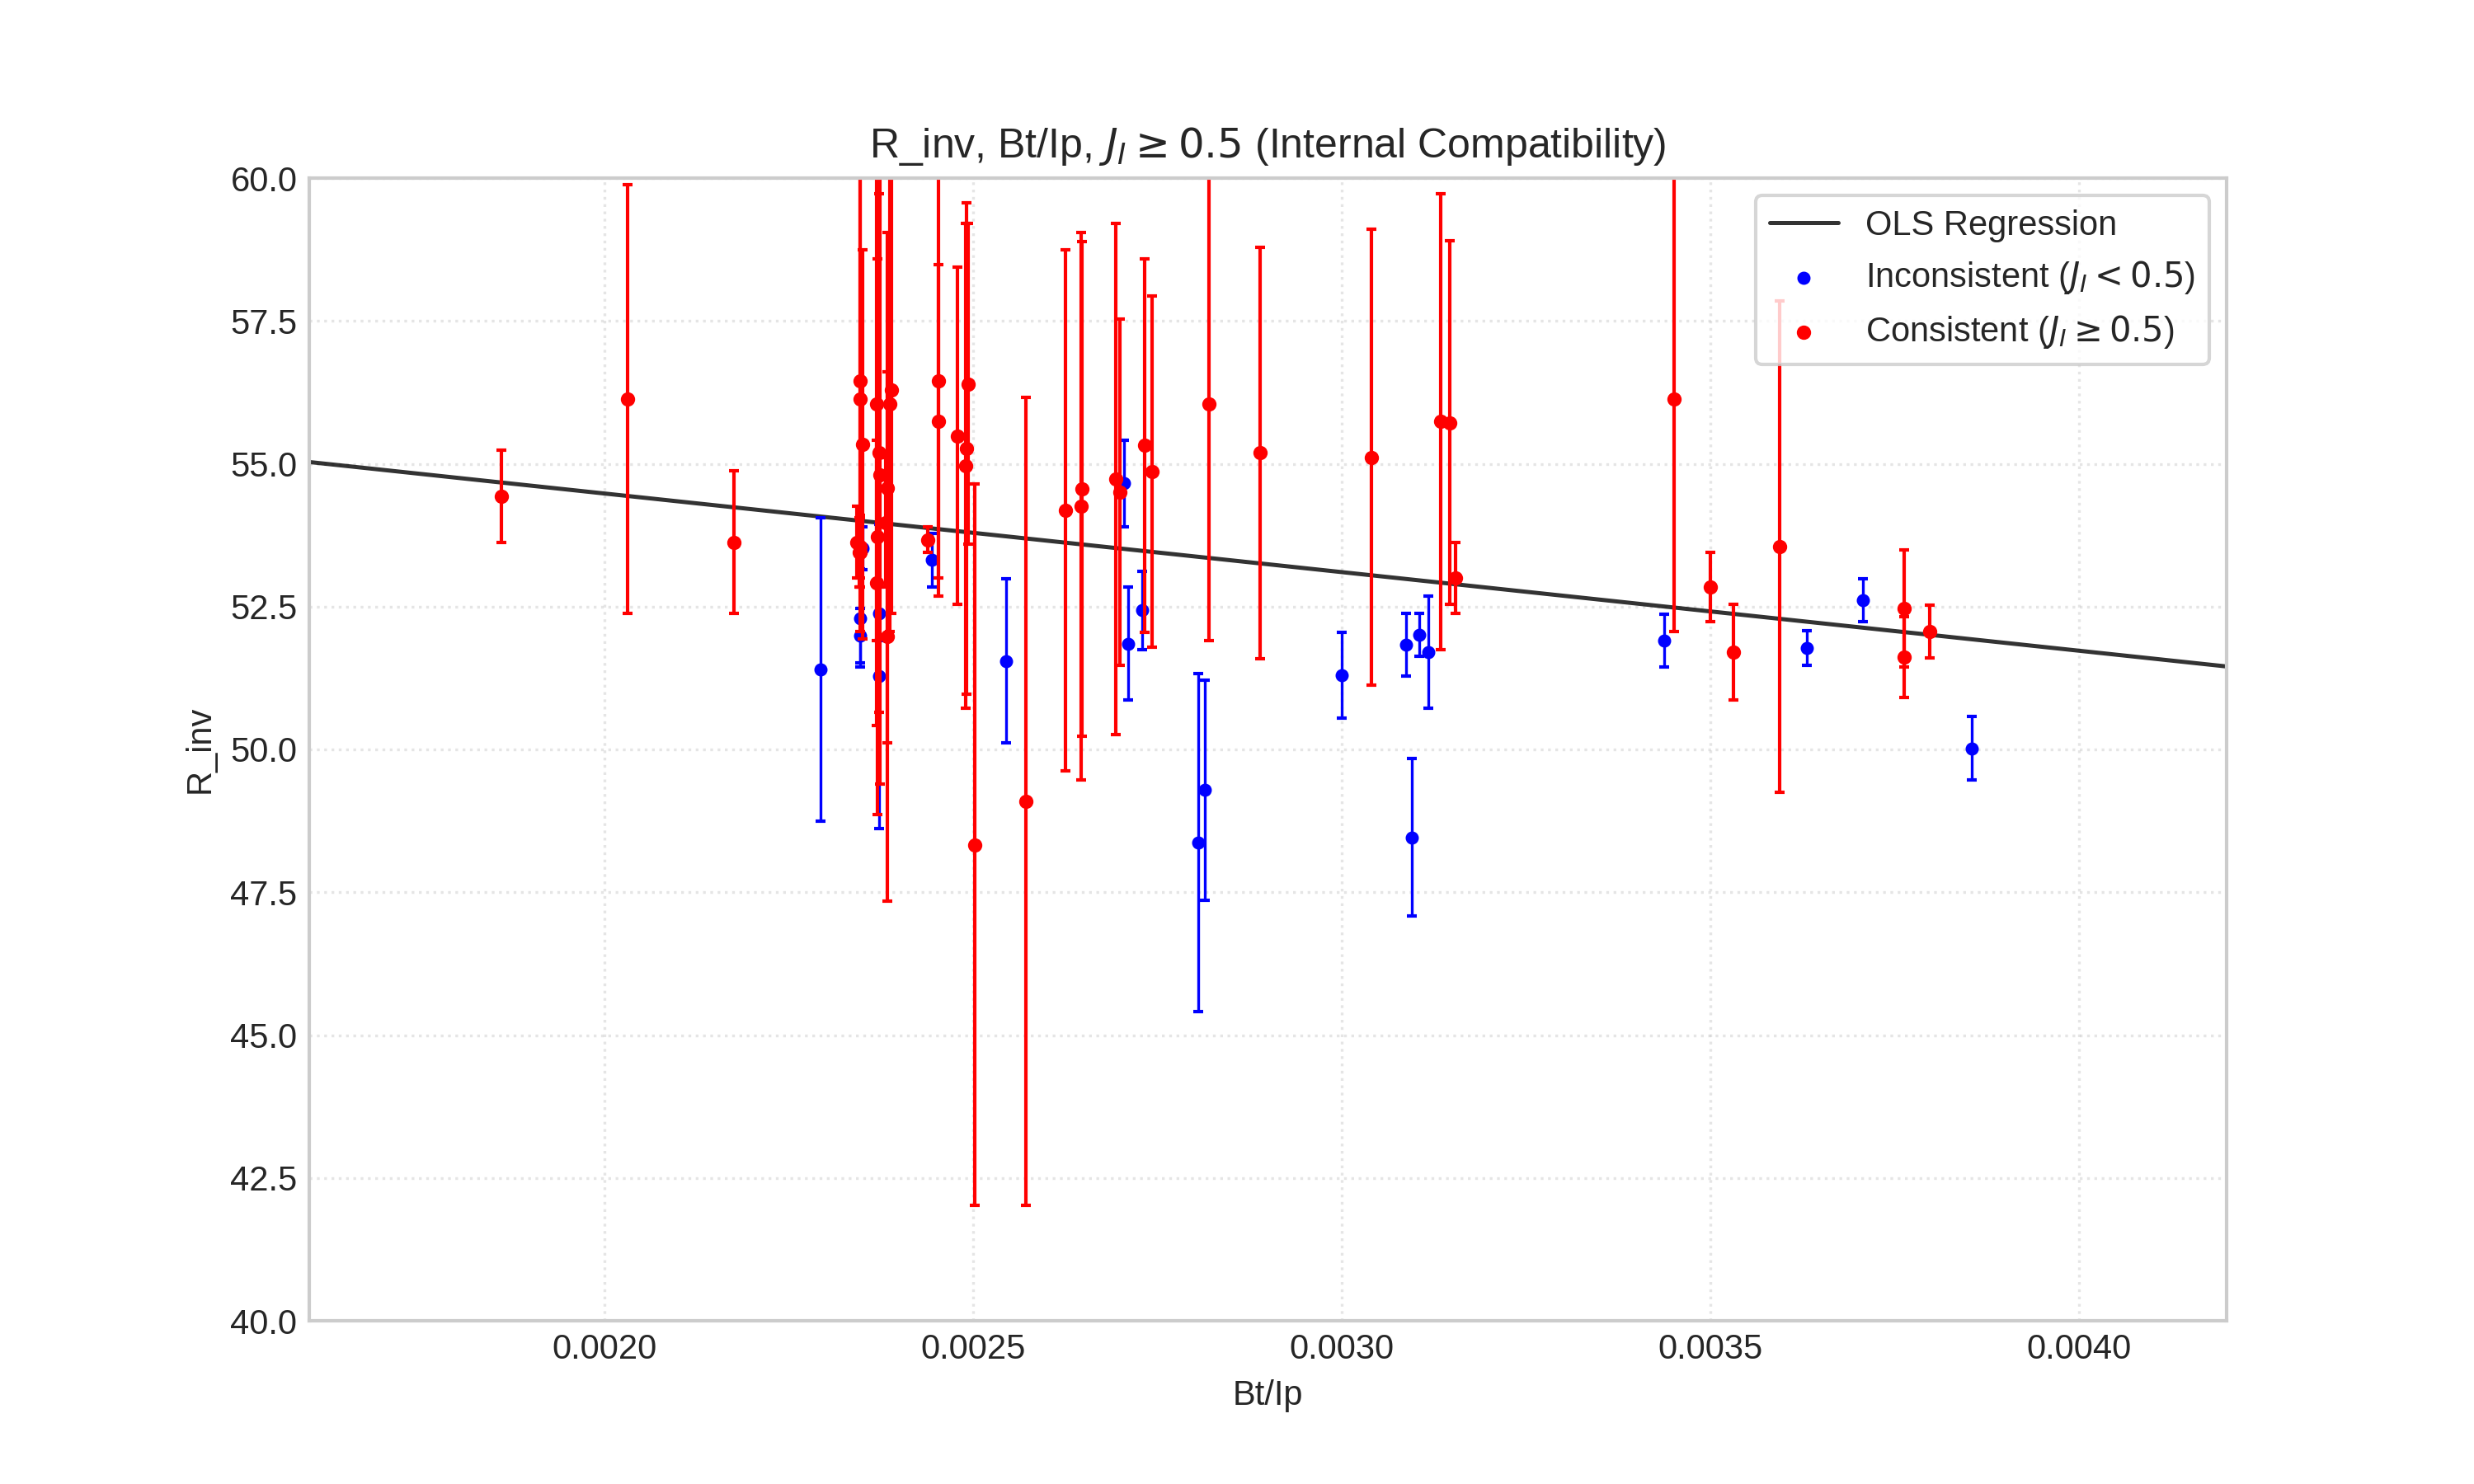
\includegraphics[width=0.8\textwidth]{images/fig_3_4_internal.png}
    \caption{Внутренние интервальные оценки инверсий ($\text{J}_I \ge 0.5$).}
    \label{fig:internal}
\end{figure}

\begin{figure}[H]
    \centering
    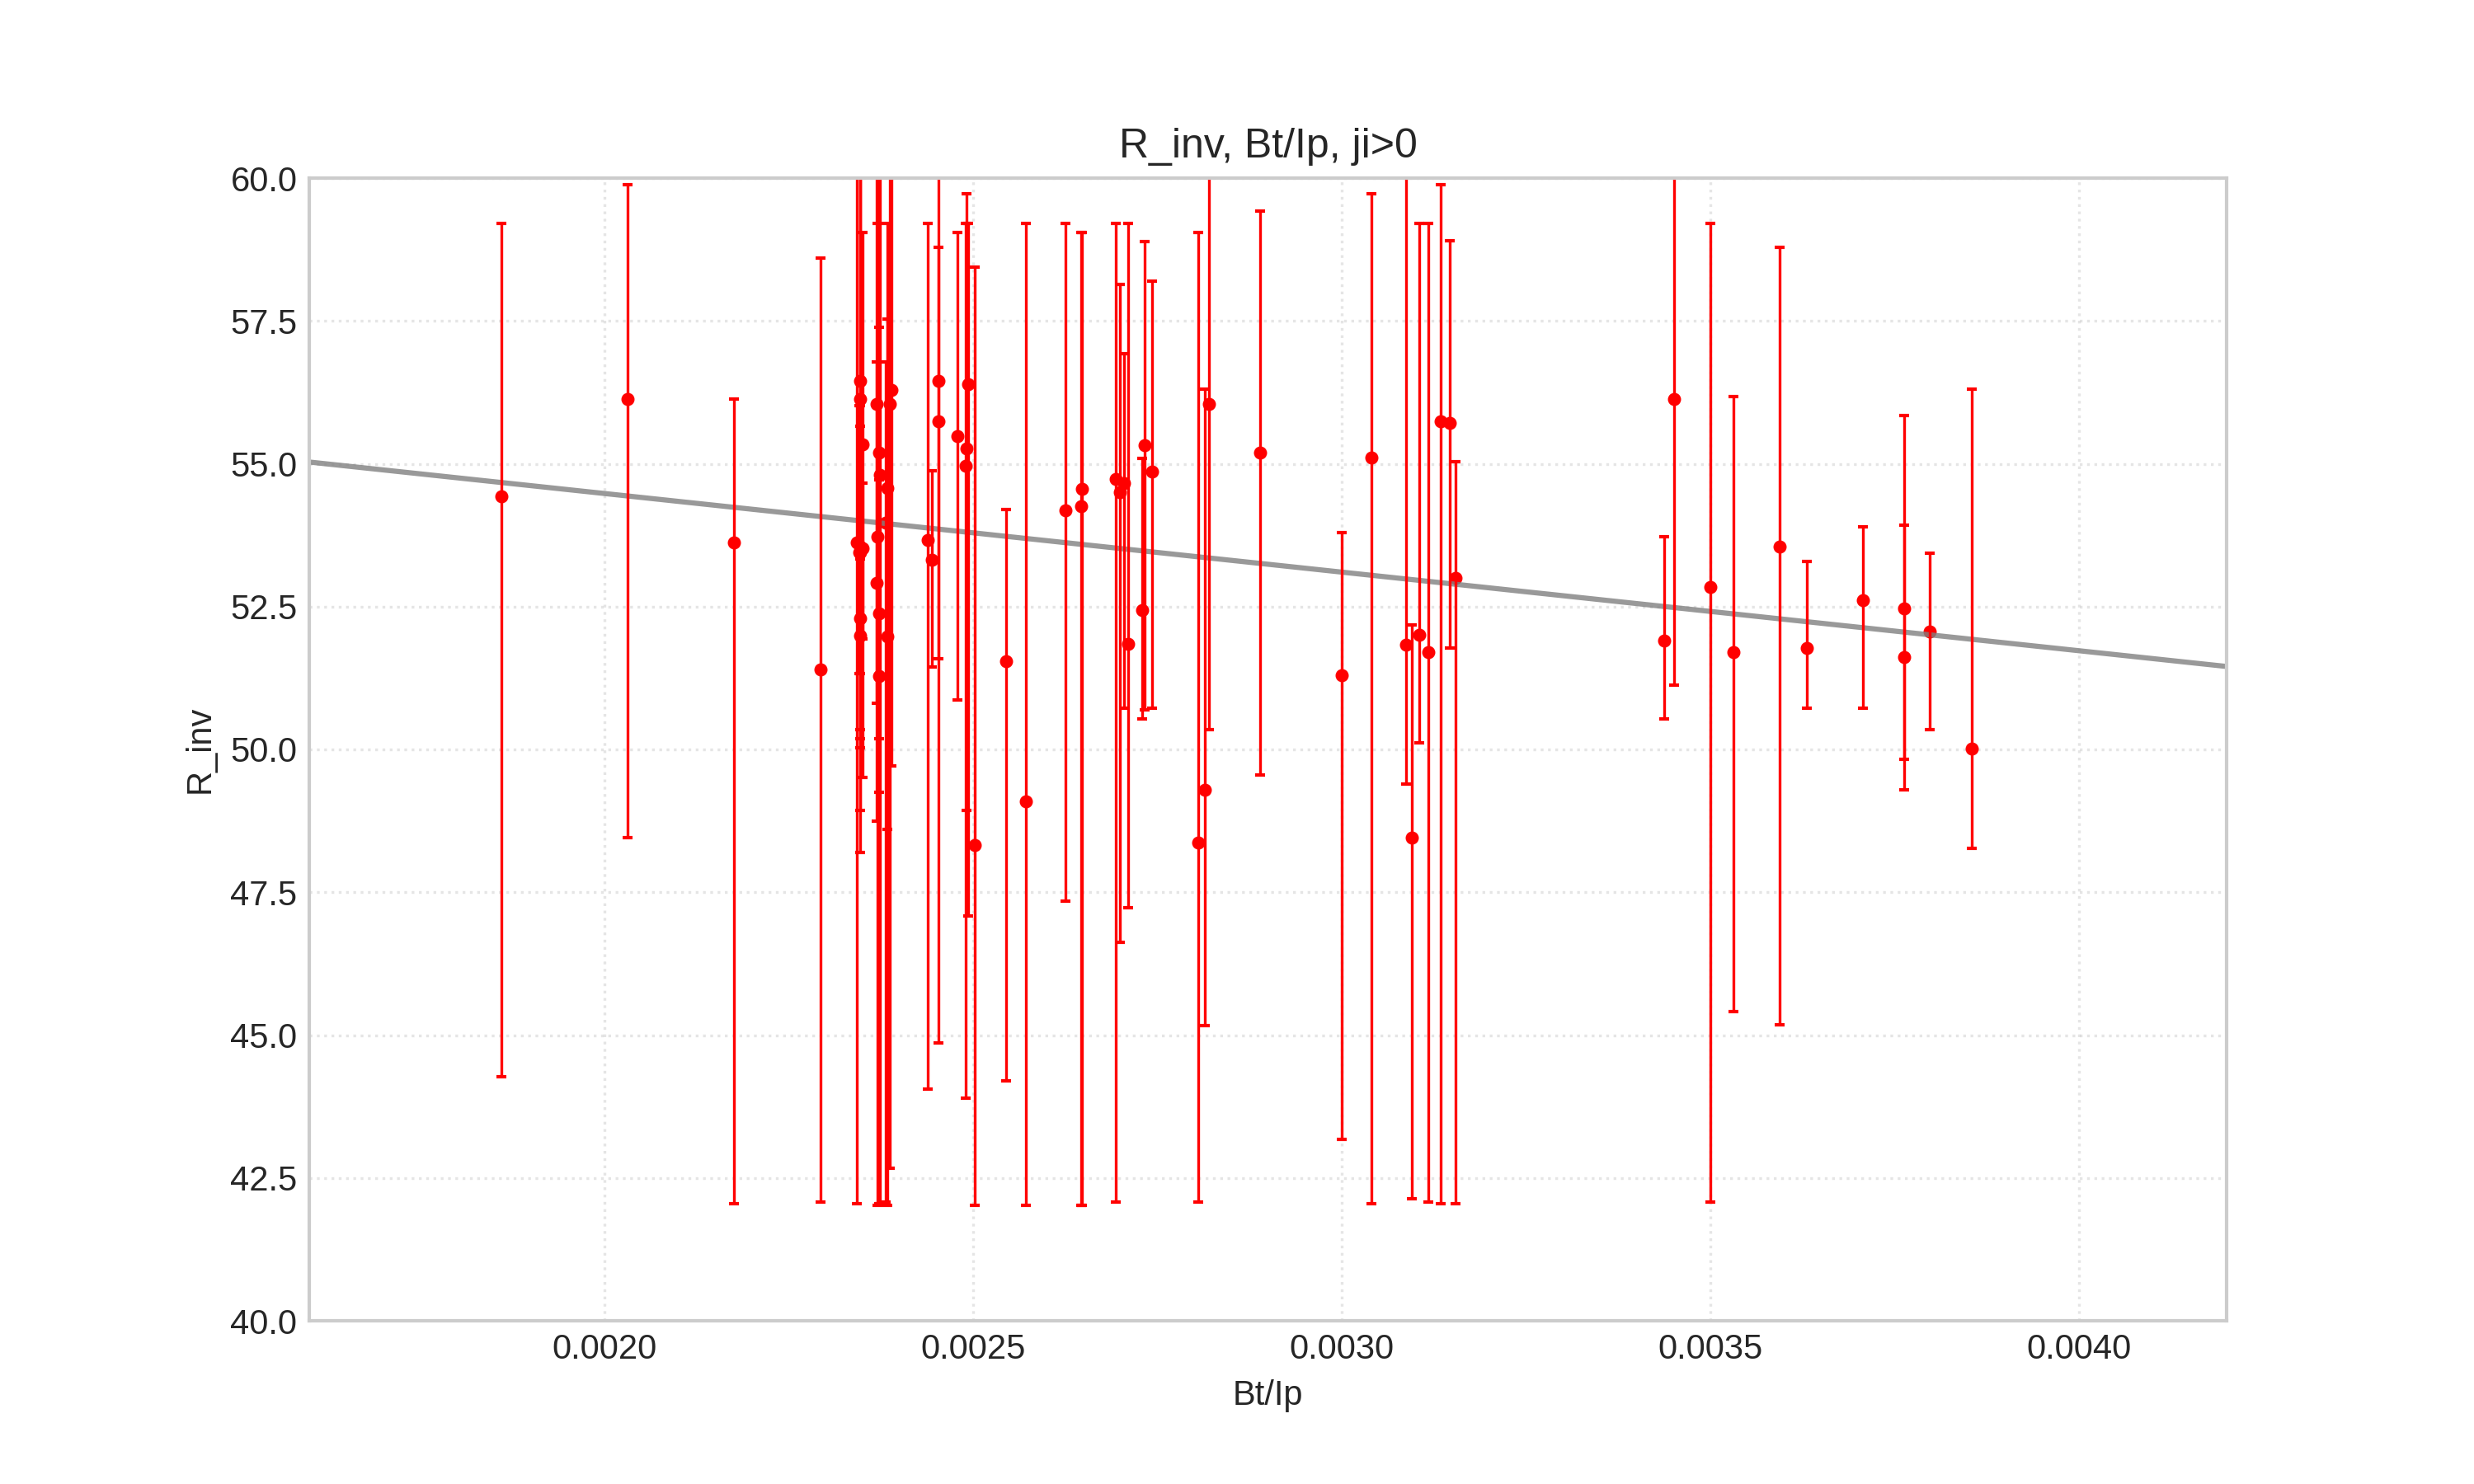
\includegraphics[width=0.8\textwidth]{images/fig_3_5_external.png}
    \caption{Внешние интервальные оценки инверсий ($\text{J}_I > 0$).}
    \label{fig:external}
\end{figure}

\subsection{Сравнительный анализ оценок}
Основные наблюдаемые особенности полученных интервальных оценок:
\begin{itemize}             
    \item \textbf{Ширина интервалов:} Внутренняя оценка дает более узкий интервал по сравнению с внешней. Среднее отношение ширины интервалов составляет $\frac{wid(R_{int})}{wid(R_{ext})} \approx 0.45$ для рассматриваемой выборки событий.
    \item \textbf{Накрывающие свойства:} Внешняя оценка является накрывающей, что гарантирует попадание в нее истинного значения параметра с высокой достоверностью. Внутренняя оценка указывает область наиболее вероятного расположения искомого значения.
    \item \textbf{Зависимость от параметров:} Обе оценки демонстрируют монотонное убывание $R_{inv}$ с ростом отношения $B_T/I_P$. Расчетный наклон регрессионной зависимости составляет:
    \begin{equation}
        \frac{dR_{inv}}{d(B_T/I_P)} \approx -1370 \pm 1000 \text{ см} / (\text{Тл/кА})
    \end{equation}
\end{itemize}

\subsection{Физическая интерпретация}
Полученные результаты позволяют сделать следующие выводы о поведении радиуса инверсии:
\begin{itemize}
    \item Тенденция к уменьшению $R_{inv}$ с ростом $B_T/I_P$ согласуется с теоретическими моделями, связывающими размер области перемешивания с конфигурацией магнитного поля.
    \item Различие в ширине интервалов отражает фундаментальный компромисс между точностью оценки (внутренний метод) и достоверностью покрытия (внешний метод).
\end{itemize}

\subsection{Информационное множество параметров}
Множество оценок параметров искомой зависимости $(\beta_1, \beta_2)$, удовлетворяющих всем интервальным ограничениям, образует информационное множество задачи. Поскольку система ограничений линейна, данное множество представляет собой выпуклый многогранник в пространстве параметров.

На рис. \ref{fig:info_set} представлено внешнее информационное множество, построенное по результатам анализа внешних интервальных оценок инверсии. Любой точке этого множества соответствует прямая, полностью лежащая внутри коридора совместных зависимостей.

\begin{figure}[H]
    \centering
    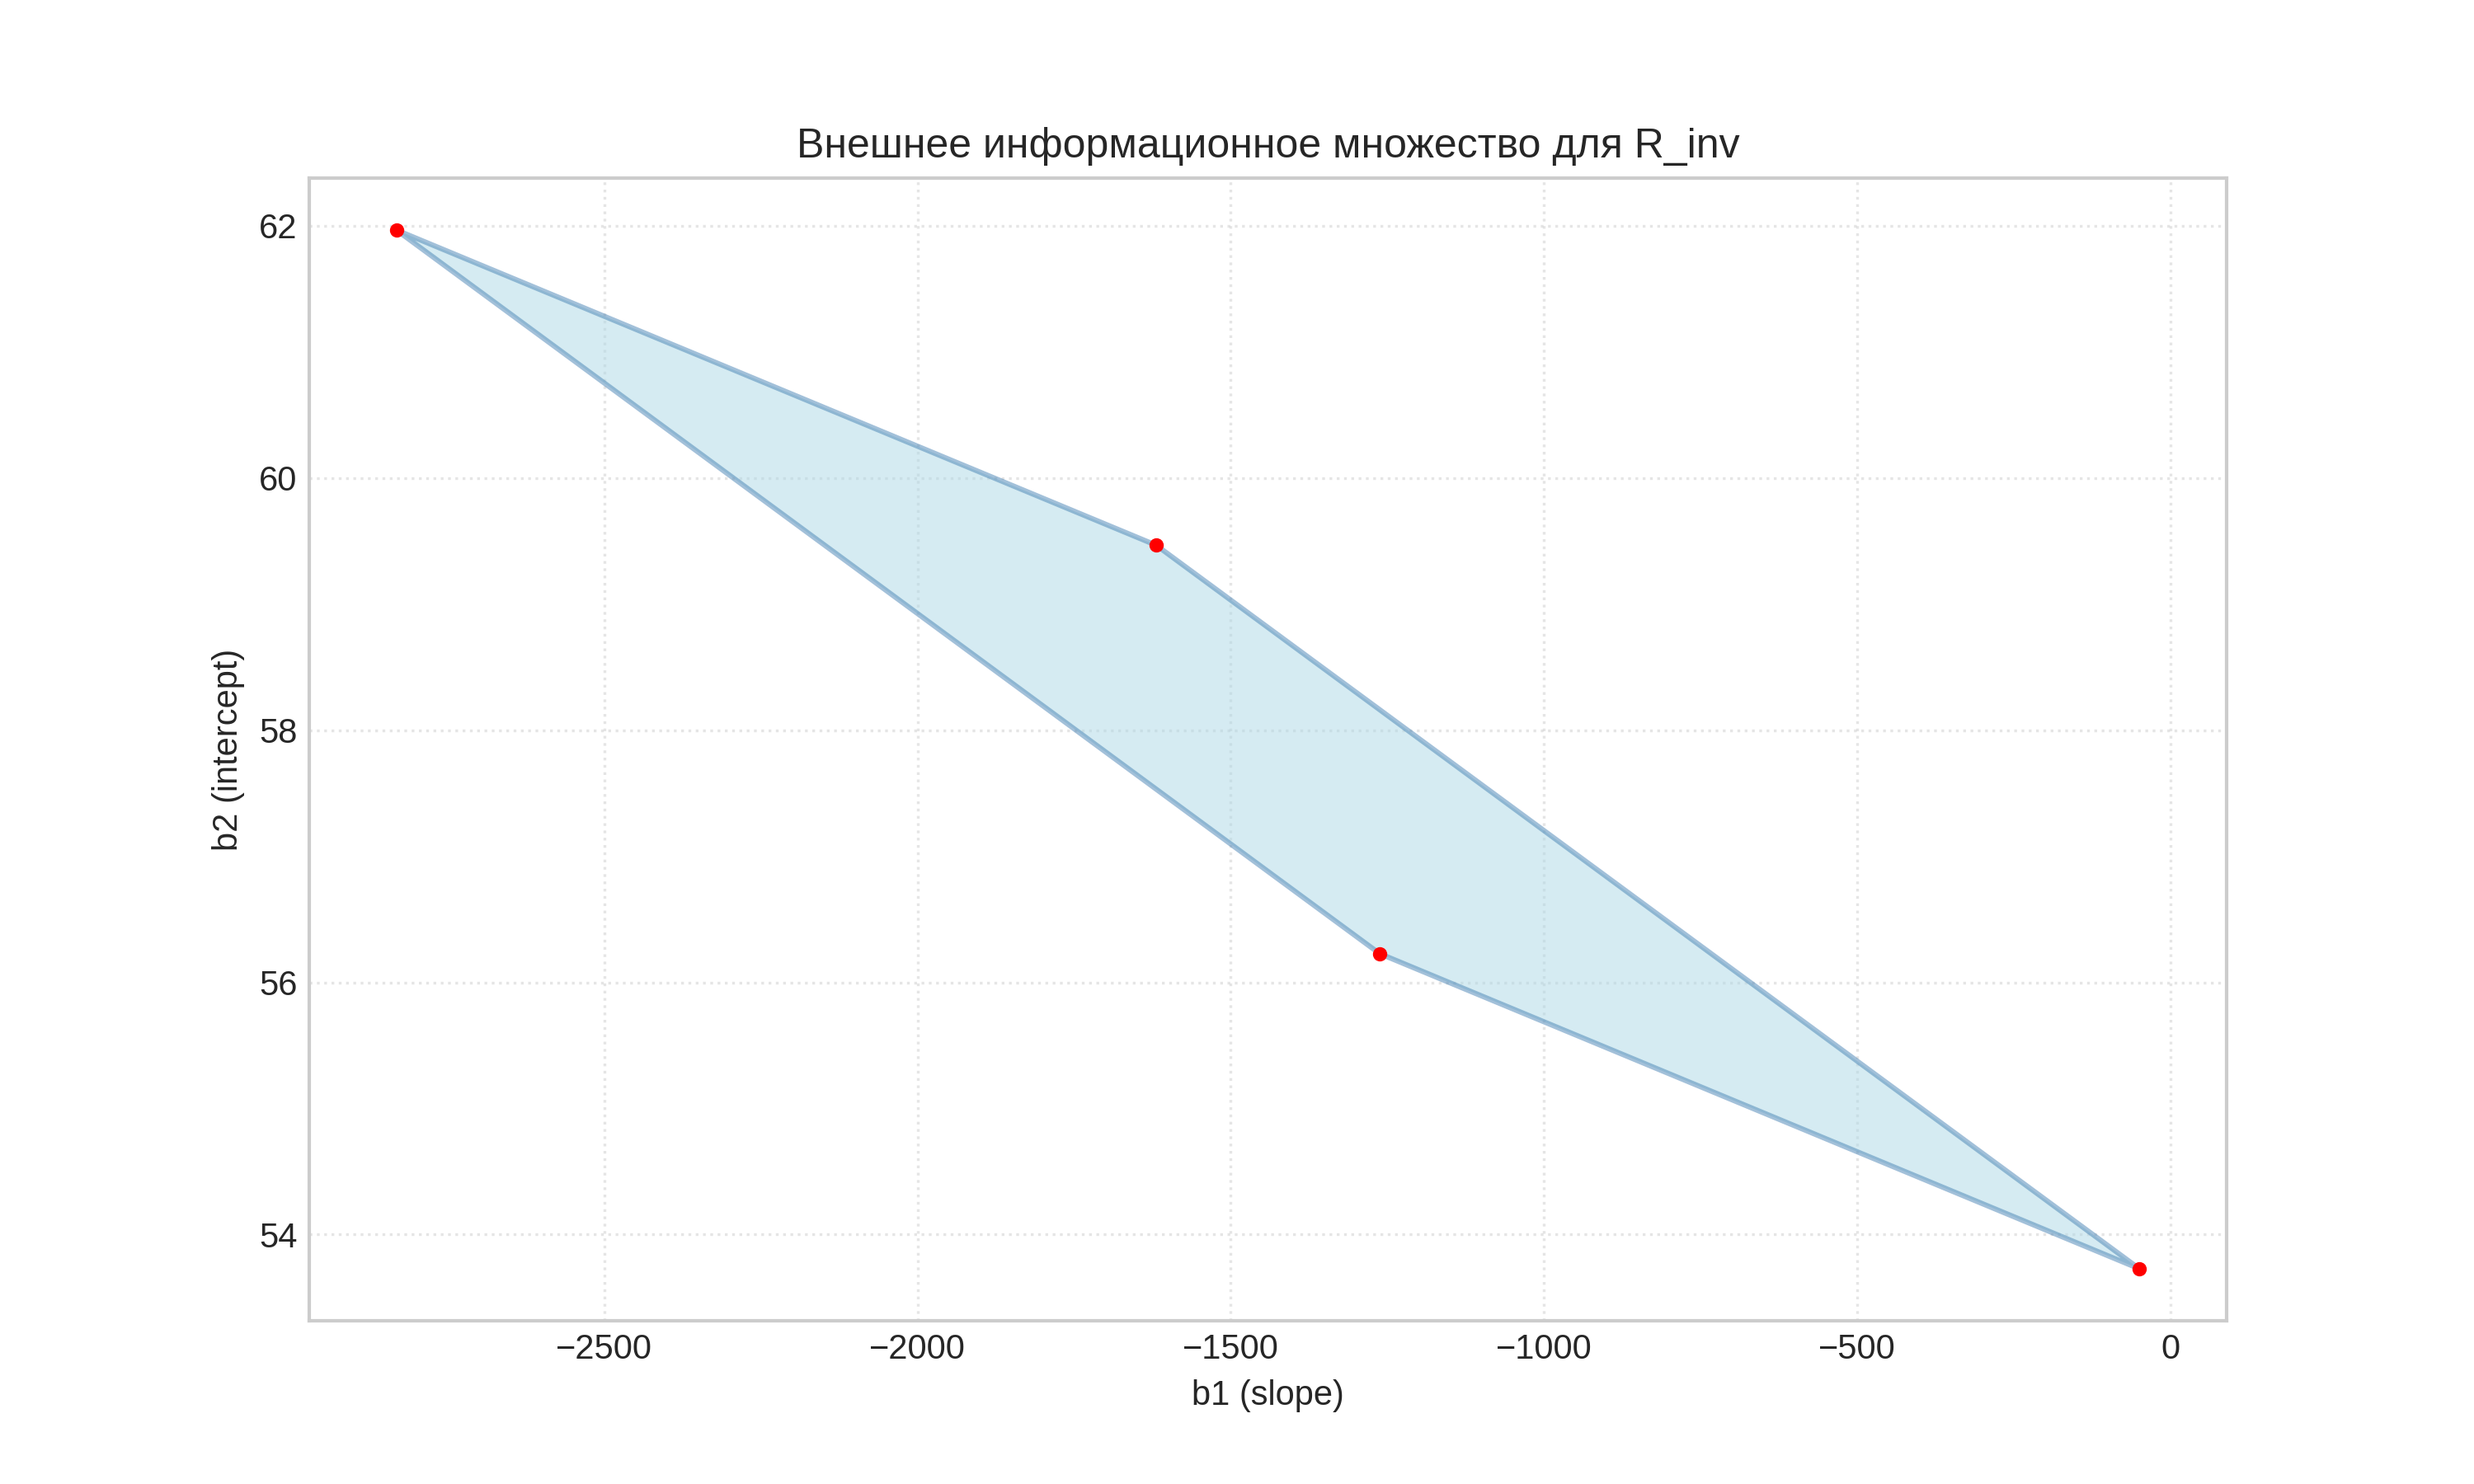
\includegraphics[width=0.8\textwidth]{images/fig_3_7_info_set.png}
    \caption{Внешнее информационное множество для $R_{inv}$ в пространстве параметров (наклон и смещение).}
    \label{fig:info_set}
\end{figure}

\subsection{Построение коридора совместных зависимостей}
Для получения итогового прогноза и оценки области неопределенности используется метод построения коридора совместных зависимостей (метод построения огибающих). Данный подход позволяет построить огибающую всех линейных зависимостей, согласующихся с экспериментальными интервальными данными.

Процедура построения состоит из следующих этапов:
\begin{enumerate}
    \item \textbf{Генерация кандидатных параметров:} На основе обучающей выборки пар $\{ (x_i, Y_i) \}_{i=1}^n$ формируется набор прямых, проходящих через границы любых двух интервалов выборки. Для каждой пары индексов $(i, j)$ рассматриваются 4 комбинации граничных точек: $(x_i, y_i^{low/high})$ и $(x_j, y_j^{low/high})$.
    \item \textbf{Проверка на допустимость:} Параметры прямой $(a, b)$ считаются допустимыми, если соответствующая прямая проходит через все интервалы выборки: $ax_k + b \in Y_k$ для всех $k=1 \dots n$. Совокупность таких параметров образует \textit{информационное множество}.
    \item \textbf{Нахождение огибающих:} Границы искомого коридора в каждой точке $x$ определяются как область значений всех допустимых прямых:
    \begin{equation}
        Y_{corr}(x) = [\min_{(a,b) \in \mathcal{I}} (ax+b), \max_{(a,b) \in \mathcal{I}} (ax+b)]
    \end{equation}
\end{enumerate}

Итоговый коридор для внешних оценок представлен на рис. \ref{fig:corridor}. Внутри области допустимых решений выделены две характерные регрессионные зависимости:
\begin{itemize}
    \item \textbf{Центр масс информационного множества} (черная линия) --- усредненная модель, минимизирующая влияние локальных экстремумов отдельных интервалов.
    \item \textbf{Центр наибольшей диагонали} (зеленая линия) --- геометрический центр прямоугольной оболочки информационного множества, представляющий наиболее устойчивое решение.
\end{itemize}

\begin{figure}[H]
    \centering
    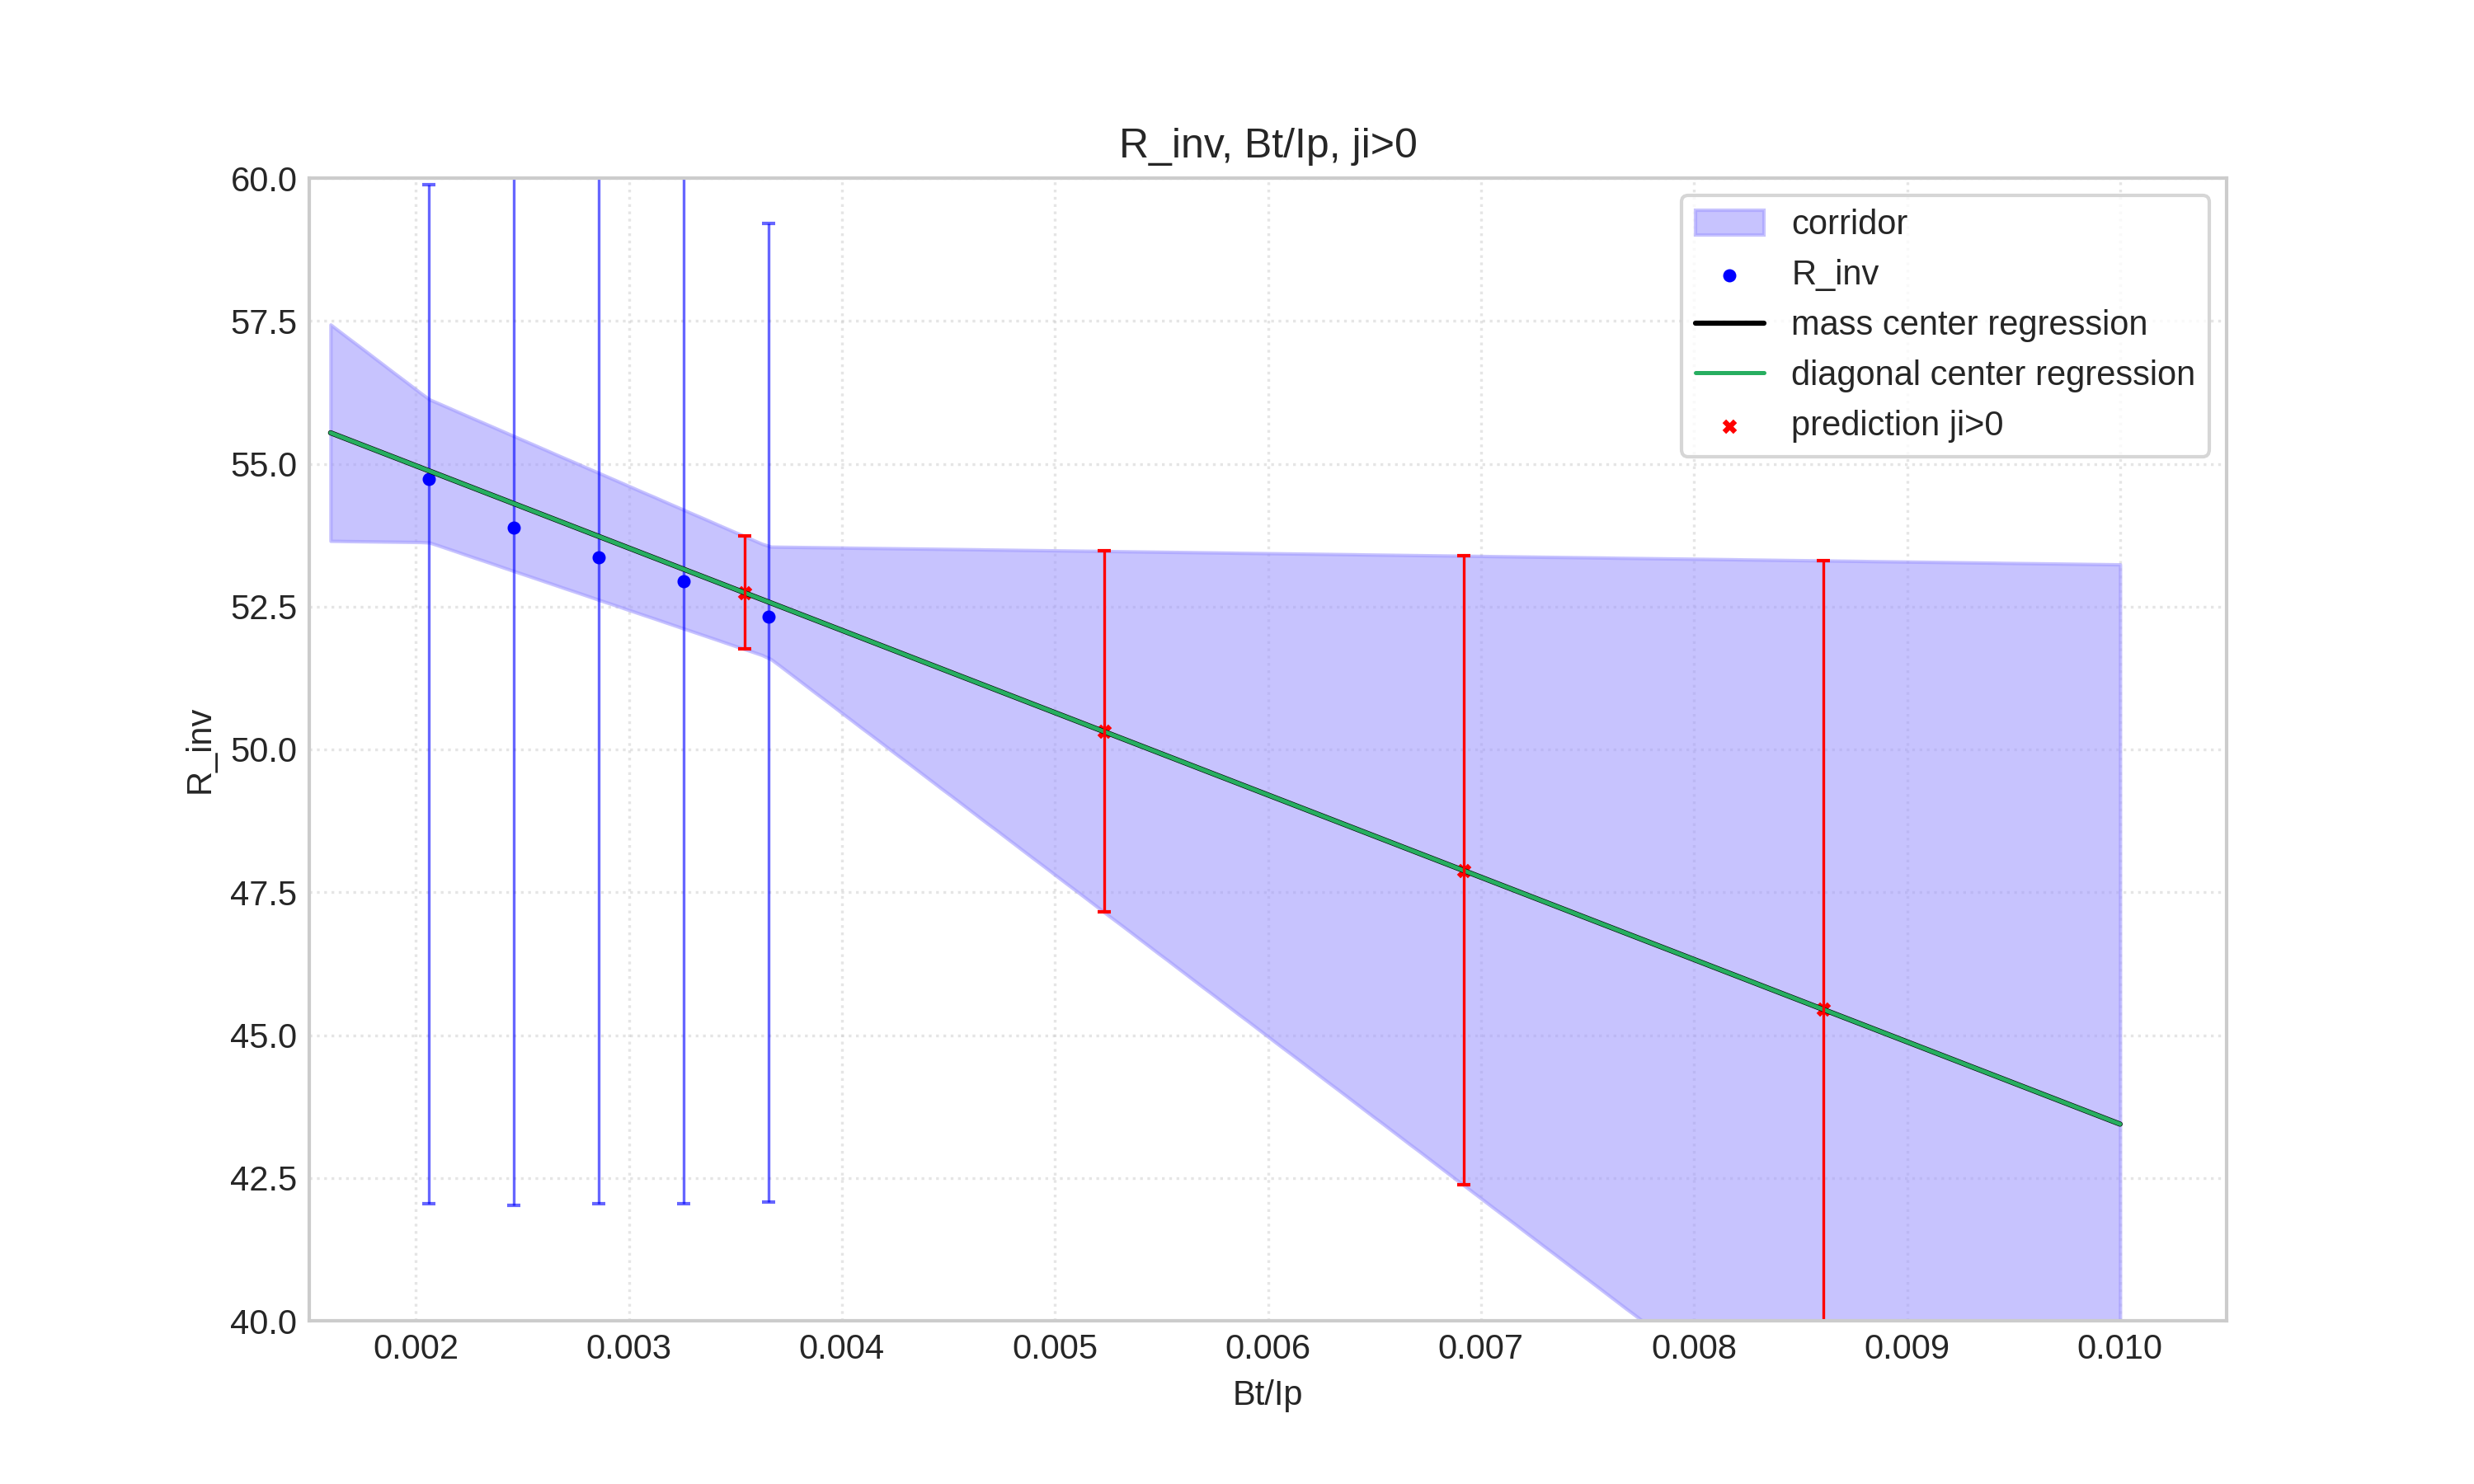
\includegraphics[width=0.85\textwidth]{images/fig_3_6_corridor.png}
    \caption{Коридор совместных зависимостей и примеры регрессий. Синяя область --- огибающая всех допустимых прямых, красные маркеры --- прогноз для экстремальных значений $B_T/I_P$.}
    \label{fig:corridor}
\end{figure}

\section{Выводы}
Разработанный программный комплекс на языке Rust позволяет проводить автоматизированный интервальный анализ данных токамака Глобус-М2. Метод построения коридора совместных зависимостей обеспечивает высокую надежность прогнозирования радиуса инверсии в новых режимах работы установки.

\end{document}
